% THIS IS SIGPROC-SP.TEX - VERSION 3.1
% WORKS WITH V3.2SP OF ACM_PROC_ARTICLE-SP.CLS
% APRIL 2009
%
% It is an example file showing how to use the 'acm_proc_article-sp.cls' V3.2SP
% LaTeX2e document class file for Conference Proceedings submissions.
% ----------------------------------------------------------------------------------------------------------------
% This .tex file (and associated .cls V3.2SP) *DOES NOT* produce:
%       1) The Permission Statement
%       2) The Conference (location) Info information
%       3) The Copyright Line with ACM data
%       4) Page numbering
% ---------------------------------------------------------------------------------------------------------------
% It is an example which *does* use the .bib file (from which the .bbl file
% is produced).
% REMEMBER HOWEVER: After having produced the .bbl file,
% and prior to final submission,
% you need to 'insert'  your .bbl file into your source .tex file so as to provide
% ONE 'self-contained' source file.
%
% Questions regarding SIGS should be sent to
% Adrienne Griscti ---> griscti@acm.org
%
% Questions/suggestions regarding the guidelines, .tex and .cls files, etc. to
% Gerald Murray ---> murray@hq.acm.org
%
% For tracking purposes - this is V3.1SP - APRIL 2009

\documentclass{acm_proc_article-sp}

\usepackage{url}
\usepackage{graphicx}

\makeatletter
\def\@copyrightspace{\relax}
\makeatother

\begin{document}

\title{I523: Project 042: Prediction of Accident prone areas}
%ubtitle{[Extended Abstract]}

\numberofauthors{4} 
\author{
\alignauthor
Nandini Goswami\\
F16-IG-3007\\
       \affaddr{Indiana University}\\
       \affaddr{Bloomington}\\
       \email{goswamin@iu.edu}
\alignauthor
Sarita Bhateja\\
F16-IG-3003\\
       \affaddr{Indiana University}\\
       \affaddr{Bloomington}\\
       \email{sbhateja@iu.edu}
\and % go to new row
\alignauthor
Kavya Guruprasad\\
F16-IG-3008\\
       \affaddr{Indiana University}\\
       \affaddr{Bloomington}\\
       \email{prasadk@iu.edu}
}

%\date{20 April 2013}


\maketitle
\begin{abstract}

The paper discusses the prediction of road accidents. We have UK road accident dataset for year the 2015. The problem is treated as a machine learning classification problem and the outcome is classified as severity of accident on a range of 1-3 where 1 is the least severe and 3 is the most severe. \\
The results have been visualized using bar graphs, line chart, histogram etc. Also, the location of various accident prone areas have been plotted on map. The data related to latitude and longitude of such locations in the dataset helped to achieve it.
  
\end{abstract}

\section{Introduction}
Every day a number of people die out of road accidents all over the world. The severity of road accidents is more in densely populated countries. A country's asset is their population and the health and safety of it is every country's top priority. Below is the statistics of Annual Global Road Crash: \cite{statistics}
\begin{itemize}
    \item Nearly 1.3 million people die in road crashes each year, on average 3,287 deaths a day.
    \item An additional 20-50 million are injured or disabled.
    \item More than half of all road traffic deaths occur among young adults ages 15-44.
    \item Road traffic crashes rank as the 9th leading cause of death and account for 2.2% of all deaths globally.
    \item Road crashes are the leading cause of death among young people ages 15-29, and the second leading cause of death worldwide among young people ages 5-14.
    \item Each year nearly 400,000 people under 25 die on the world's roads, on average over 1,000 a day.
    \item Over 90 percent of all road fatalities occur in low and middle-income countries, which have less than half of the world's vehicles.
    \item Road crashes cost USD 518 billion globally, costing individual countries from 1-2 percent of their annual GDP.
    \item Road crashes cost low and middle-income countries USD 65 billion annually, exceeding the total amount received in developmental assistance.
    \item Unless action is taken, road traffic injuries are predicted to become the fifth leading cause of death by 2030.
\end{itemize}
The numbers are startling and there is alarming need to have control on road accidents and ensure better road safety.

This project is to predict the severity of an accident for a particular location given various factors/parameter. The analysis and classification is done of locations more prone to severe accidents. Based on the analysis, a strategy can be applied in order to make people aware of this information, this can be achieved via an phone based application as well. This information will also help tourists to understand the location in a better way and ensure safety measures while traveling. 

Additionally, we have plotted these accidents prone locations on Google map using Google map APIs in python so as to provide better visualisation of results.

The project has been implemented on python as a language using Apache Spark on Databricks as a platform.

\section{Analysis}


\subsection{Analysis of Dataset}

The dataset contains the UK road accident data for the year 2015 and has been taken from the following web-page. \cite{data-gov-uk}

The description of the columns of the dataset is below:

\begin{itemize}
    \item \texttt{Accident\char`_Index}: The first column i.e \texttt{Accident\char`_Index} acts as the unique key in the data set and helped us to map every column to its respective key. 
    \item \texttt{Location\char`_Easting\char`_OSGR}, \texttt{Location\char`_Northing\char`_OSGR}, Longitude, Latitude: The second, third, fourth and the fifth column of the dataset i.e.  Location\char`_Easting\char`_OSGR,  \texttt{Location\char`_Northing\char`_OSGR}, Longitude and Latitude gives data about the accident location. These location related data helped to plot the results on google maps.
    \item \texttt{Police\char`_Force}: The sixth column is \texttt{Police\char`_Force} that provides data related to police force at the accident location.
    \item \texttt{Accident\char`_Severity}: The seventh column is    \\ \texttt{Accident\char`_Severity}. This column suggests the severity of the accident based on numbers. A number 3 indicates a severe accident  whereas if the accident severity of 1 indicates a less severe accident. This column is acting as a class label for the classification Machine Learning algorithm.
    \item \texttt{Number\char`_of\char`_Vehicles} and \texttt{Number\char`_of\char`_Casualties}: The eighth and ninth column explains the number of vehicles involved in accident and the number of casualties occurred in the accident.
    \item Date,\texttt{Day\char`_of\char`_Week} and Time: The tenth, eleventh and twelfth column provides data about date, day and time of the accident occurring. Using these we can do analysis to find on which day of the week or time most accidents occur. 
    \item \texttt{Local\char`_Authority\char`_(District)} and \\ \texttt{Local\char`_Authority\char`_(Highway)}:The thirteenth and fourteenth column gives us the district and highway numbers. Doing analysis of these two column we can visualise which highways and districts are most prone to severe accidents. 
    \item \texttt{1st\char`_Road\char`_Class},  \texttt{1st\char`_Road\char`_Number},  \texttt{Road\char`_Type}, \\ \texttt{2nd\char`_Road\char`_Class} and  \texttt{2nd\char`_Road\char`_Number}:The fifteenth, sixteenth, seventeenth, twenty-first and twenty-second column is the road class which gives us the classification of the road.
    \item \texttt{Speed\char`_limit}:The eighteenth column is the speed limit of the road.
    \item  \texttt{Junction\char`_Detail} and \texttt{Junction\char`_Control}: The nineteenth and twentieth column gives us the junction and junction control details.
    \item \texttt{Pedestrian\char`_Crossing-Human\char`_Control} and \\ \texttt{Pedestrian\char`_Crossing-Physical\char`_Facilities}:The twenty-third and twenty-fourth column provides data about Pedestrian Crossing.
    \item \texttt{Light\char`_Conditions}: The twenty-fifth column indicates the light conditions near the accident on a scale of 1-7.
    \item \texttt{Weather\char`_Conditions}: The twenty-sixth column is the weather conditions on a scale of 1-9.
    \item \texttt{Road\char`_Surface\char`_Conditions}: The twenty-seventh column is the road-surface-condition which is of the range 1-5
    \item \texttt{Special\char`_Conditions\char`_at\char`_Site}: The twenty-eighth column indicates if there were any other conditions in the accident sight which might have caused the accident and it ranges from 0-7.
    \item \texttt{Carriageway\char`_Hazards}: The twenty-ninth column is the carriageway-hazard which indicates any barriers in the road. The number ranges from 0-7.
    \item \texttt{Urban\char`_or\char`_Rural\char`_Area}:The thirtieth column determines if the road belongs to a rural or an urban area.
    \item \texttt{Did\char`_Police\char`_Officer\char`_Attend\char`_Scene\char`_of\char`_Accident}:The thirty-first column gives us information whether police came to the accident spot or not.
    \item \texttt{LSOA\char`_of\char`_Accident\char`_Location}:The thirty-second column is the LSOA OF accident location which is the geographical location surrogate for latitude and longitude. 
\end{itemize}
The feature extraction is done and as a result, few of the features were removed in order to get better result. 

\subsection{Cleaning of Dataset}

The dataset has been cleaned in order to get better result and accuracy. The null values have been removed and also, a check is in place in order to look for duplicate records. 

We have removed few features as a part of cleaning and extraction data. The features such as accident ID, location specific features, information related to post accident details, authority etc. have been removed. During the run of Machine Learining algorithm, the information related to specific location details, column with unique values hinders to generalise the information; it memorizes the data and tends to learn the specific data. As a result, it will not generalise the result when the code is run using another dataset. The location related data is helpful to visualize the results and plot the locations on google maps.\\
\\
The feature normalisation is done for feature Time so as to normalize the range of values. In the original dataset, time has comparatively wide range; normalisation is important to get better result and include Time as a feature in the algorithm. The results provide insight to accidents occurring are more at what time in the day. 

\subsection{Approach for problem statement}


The problem is treated as a Classification problem of machine learning where a dataset and corresponding class label is provided. This kind of data can be used for supervised learning.Thus, we will build a model using classification or supervised learning algorithm such as Decision tree, Naive Bayes. The model is then trained on training set and results are tested on test set.
We have implemented Decision tree and Logistic Regression for the problem. The dataset has been divided into 80 - 20 in order to train the model on 70 percent and to test on rest of the 30 percent. 

Brief overview of the Algorithms used:

\textbf{Decision Tree}: Decision tree learning is the construction of a decision tree from class-labeled training tuples. A decision tree is a flow-chart-like structure, where each internal (non-leaf) node denotes a test on an attribute, each branch represents the outcome of a test, and each leaf (or terminal) node holds a class label. The topmost node in a tree is the root node. A decision tree is a simple representation for classifying examples. The goal is to create a model that predicts the value of a target variable based on several input variables.\\
In decision analysis, a decision tree can be used to visually and explicitly represent decisions and decision making. Classification tree analysis is when the predicted outcome is the class to which the data belongs. \cite{dtree}

\textbf{Logistic Regression}: The logistic regression is a predictive analysis.  It is used to describe data and to explain the relationship between one dependent binary or multinomial variable and one or more metric independent variables.\\
Genarally, Logistic regression is the appropriate regression analysis to conduct when the dependent variable is dichotomous. Cases with more than two categories are referred to as multinomial logistic regression or, if the multiple categories are ordered, as ordinal logistic regression. \cite{logisticregression}\\
\\
We have used multinomial logistic regression as the class label has more than two values to predict. In this case, the algorithm works as one versus all others.

\subsection{Analysis of result}

\subsubsection{Analysis of Algorithm}

\textbf{Decision tree}: The dataset is split into 80-20 ratio. The 80 percent of the data i.e. the training data is fed to the decision tree classifier and a tree is returned. This tree has dept of 5. When this tree is fed with the test data for prediction, it results in an accuracy of 85 percent and the error is 15 percent approximately.
\\
\\
\textbf{Logistic Regression}: Similar to decision tree, for logistic regression we will train the model using training data and test the model created by logistic regression algorithm using test data. The result of multinomial logistic regression is similar to decision tree with accuracy as 85 percent and error of 15 percent approximately.

We implemented two algorithms to classify and compare their results to ensure that we use the algorithm which gives better performance. But on running both the algorithms we found both are giving similar performance. Both the algorithms are equally efficient for predicting whether a location a severe accident prone or not.

\subsubsection{Visualizations}

The Figure 1 shows the number of accidents occurred on the days of the week (1-Sunday through 7-Saturday). The chart shows that maximum accidents occurred on Friday.

\begin{figure}
      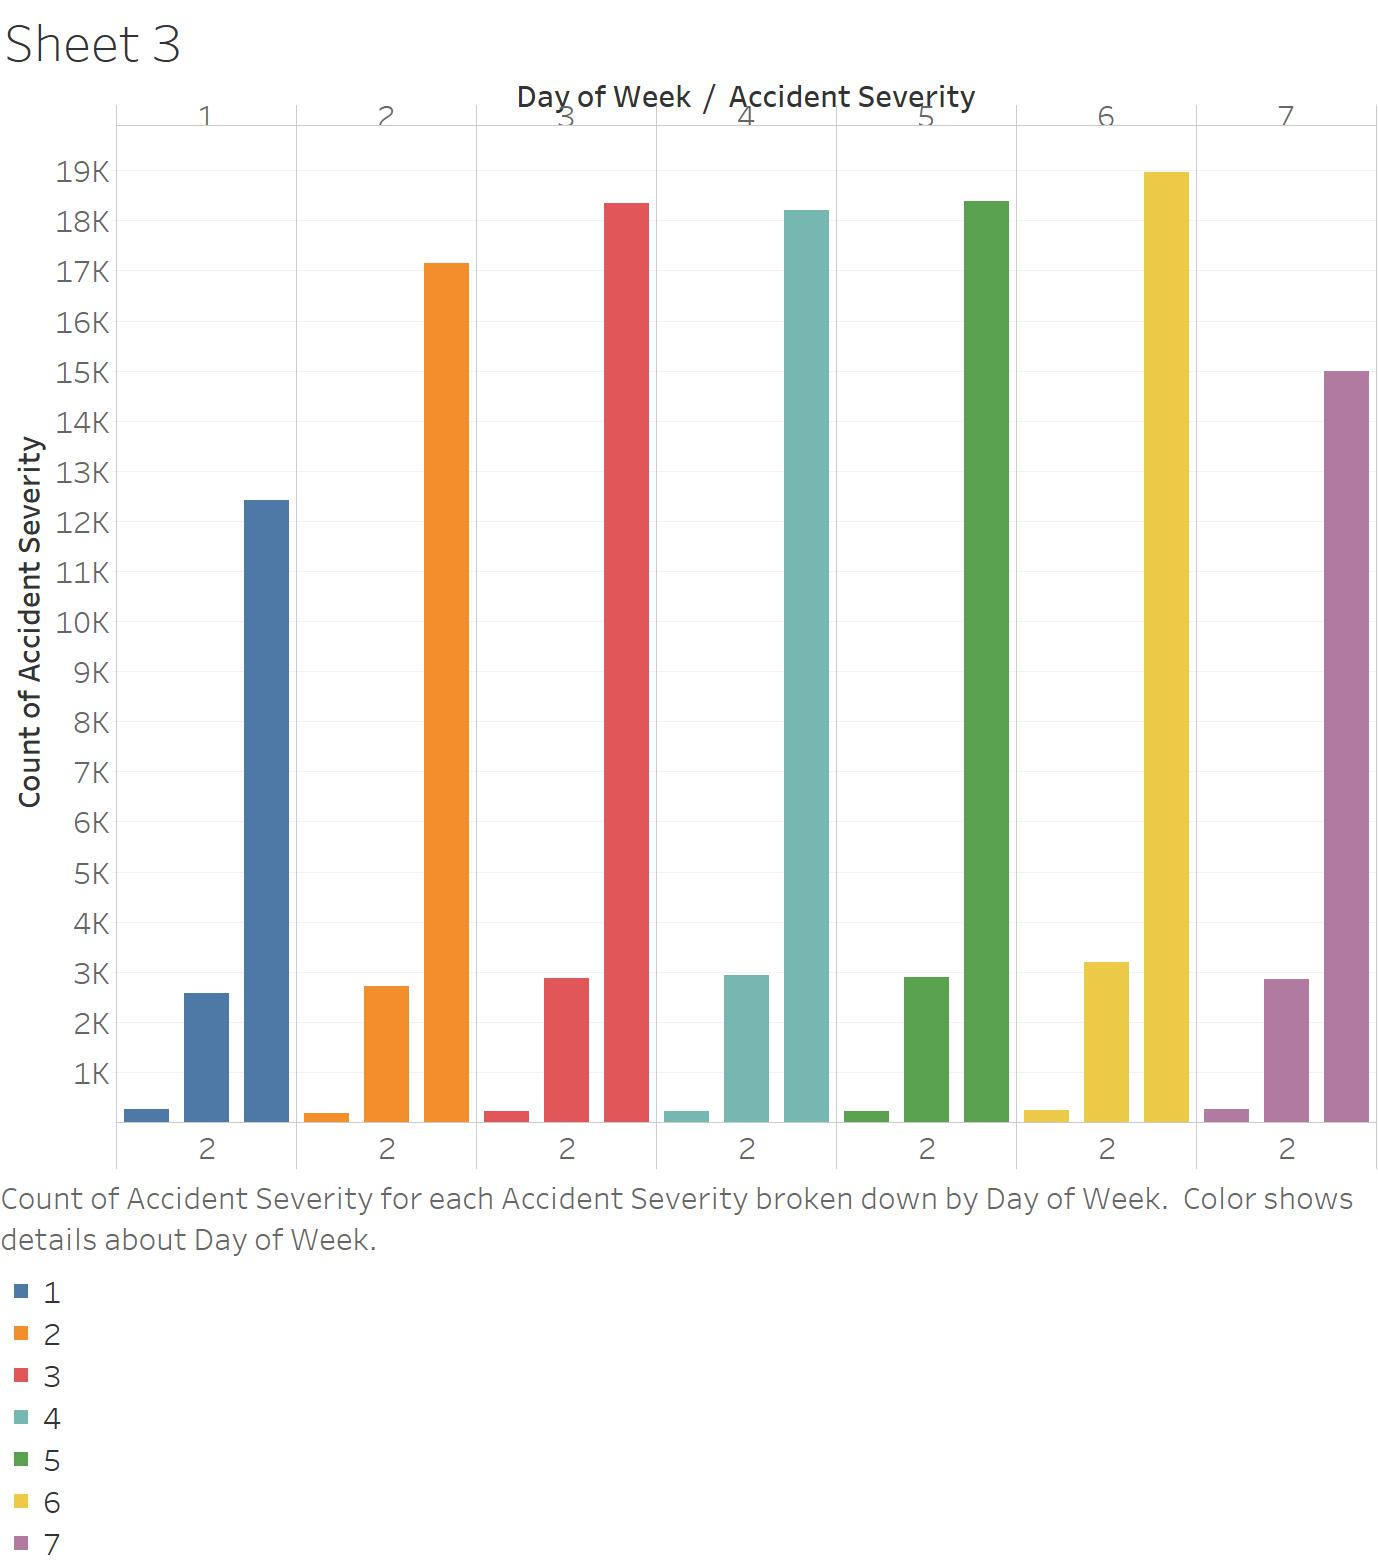
\includegraphics[width=1.0\columnwidth]{images/daysofweek.jpg}
  \caption{Number of accidents occurred on days of week}
\end{figure}

\begin{figure*}
  \centering
      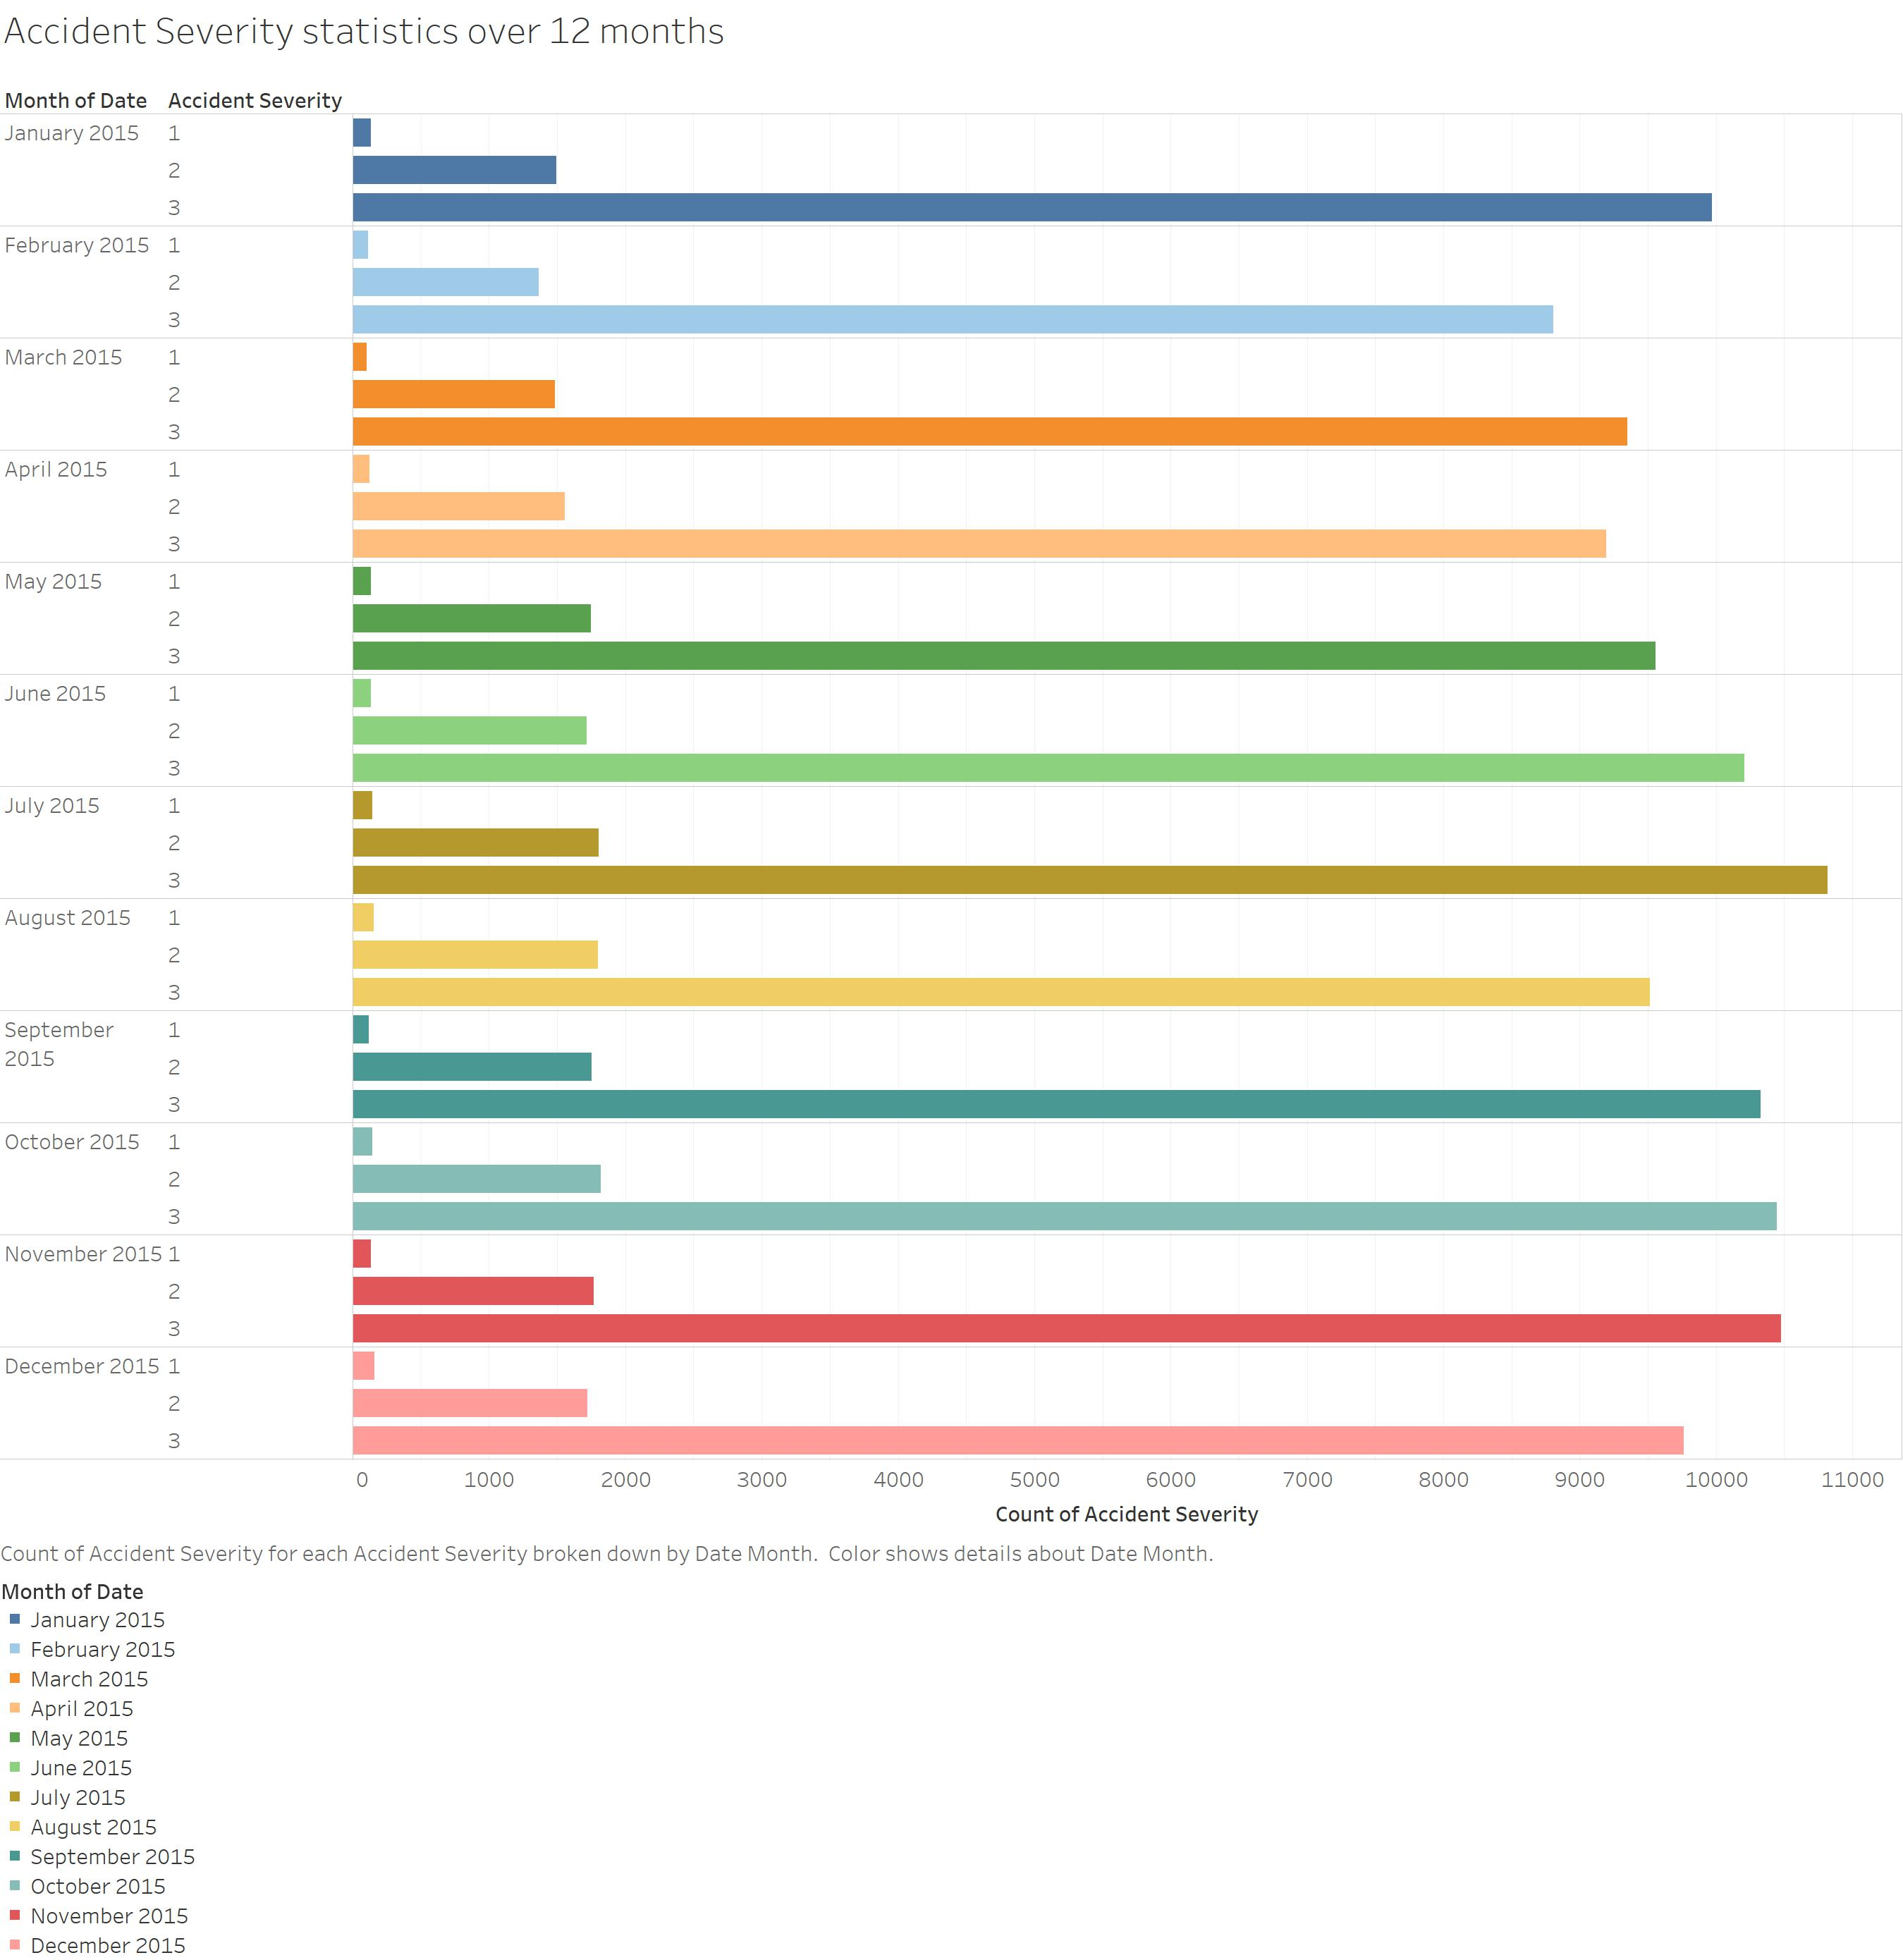
\includegraphics[width=1.0\textwidth]{images/bar.jpg}
  \caption{Accident severity with respect to months of the year.}
\end{figure*}


The Figure 2 shows the number of accidents occurring in each month with severity. The data is startling as the number of severe accidents are quite high as compared to low severity accidents with July 2015 being the highest and February 2015 being the lowest.
\\

\begin{figure}
  \centering
      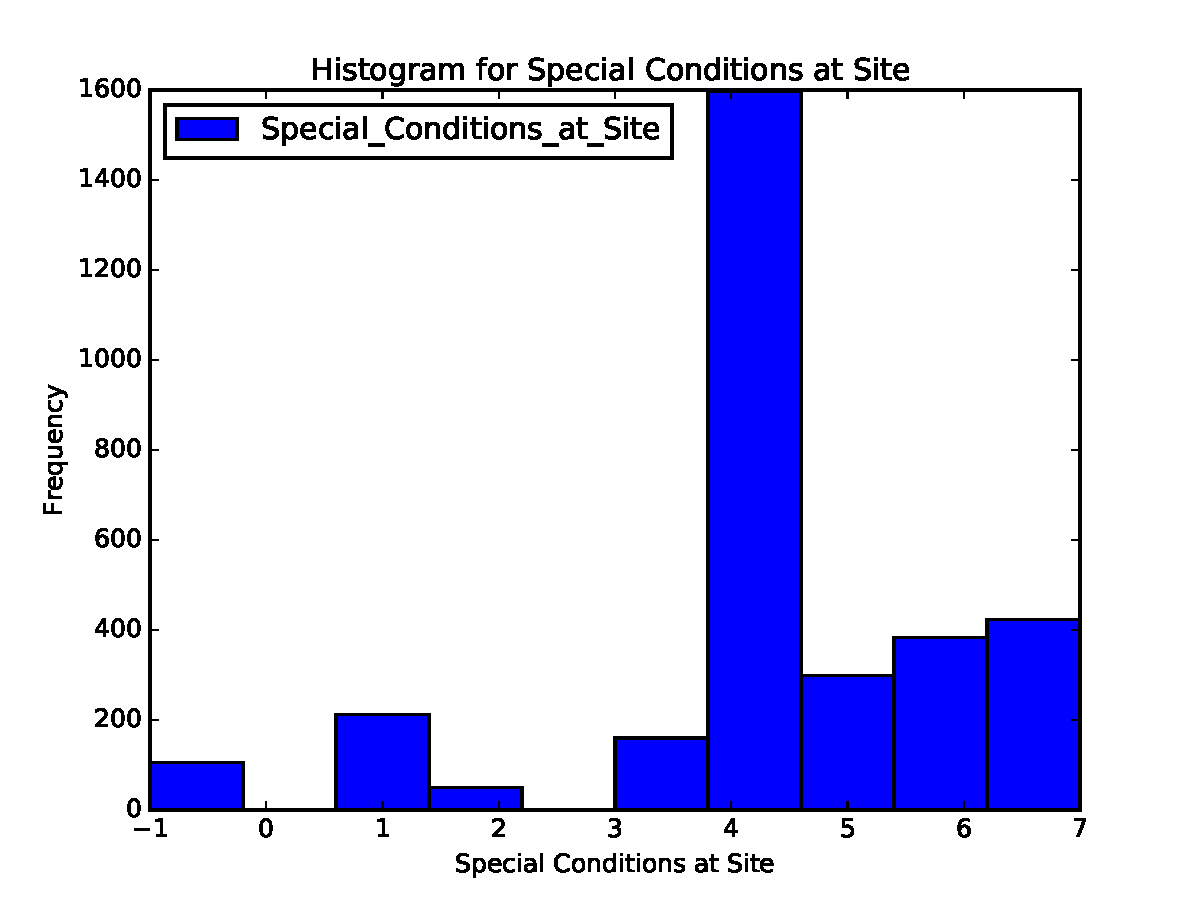
\includegraphics[width=1.0\columnwidth]{images/histogram-othconditions.pdf}
  \caption{Number of accidents occurred when other conditions were present}
\end{figure}

\begin{figure}
  \centering
      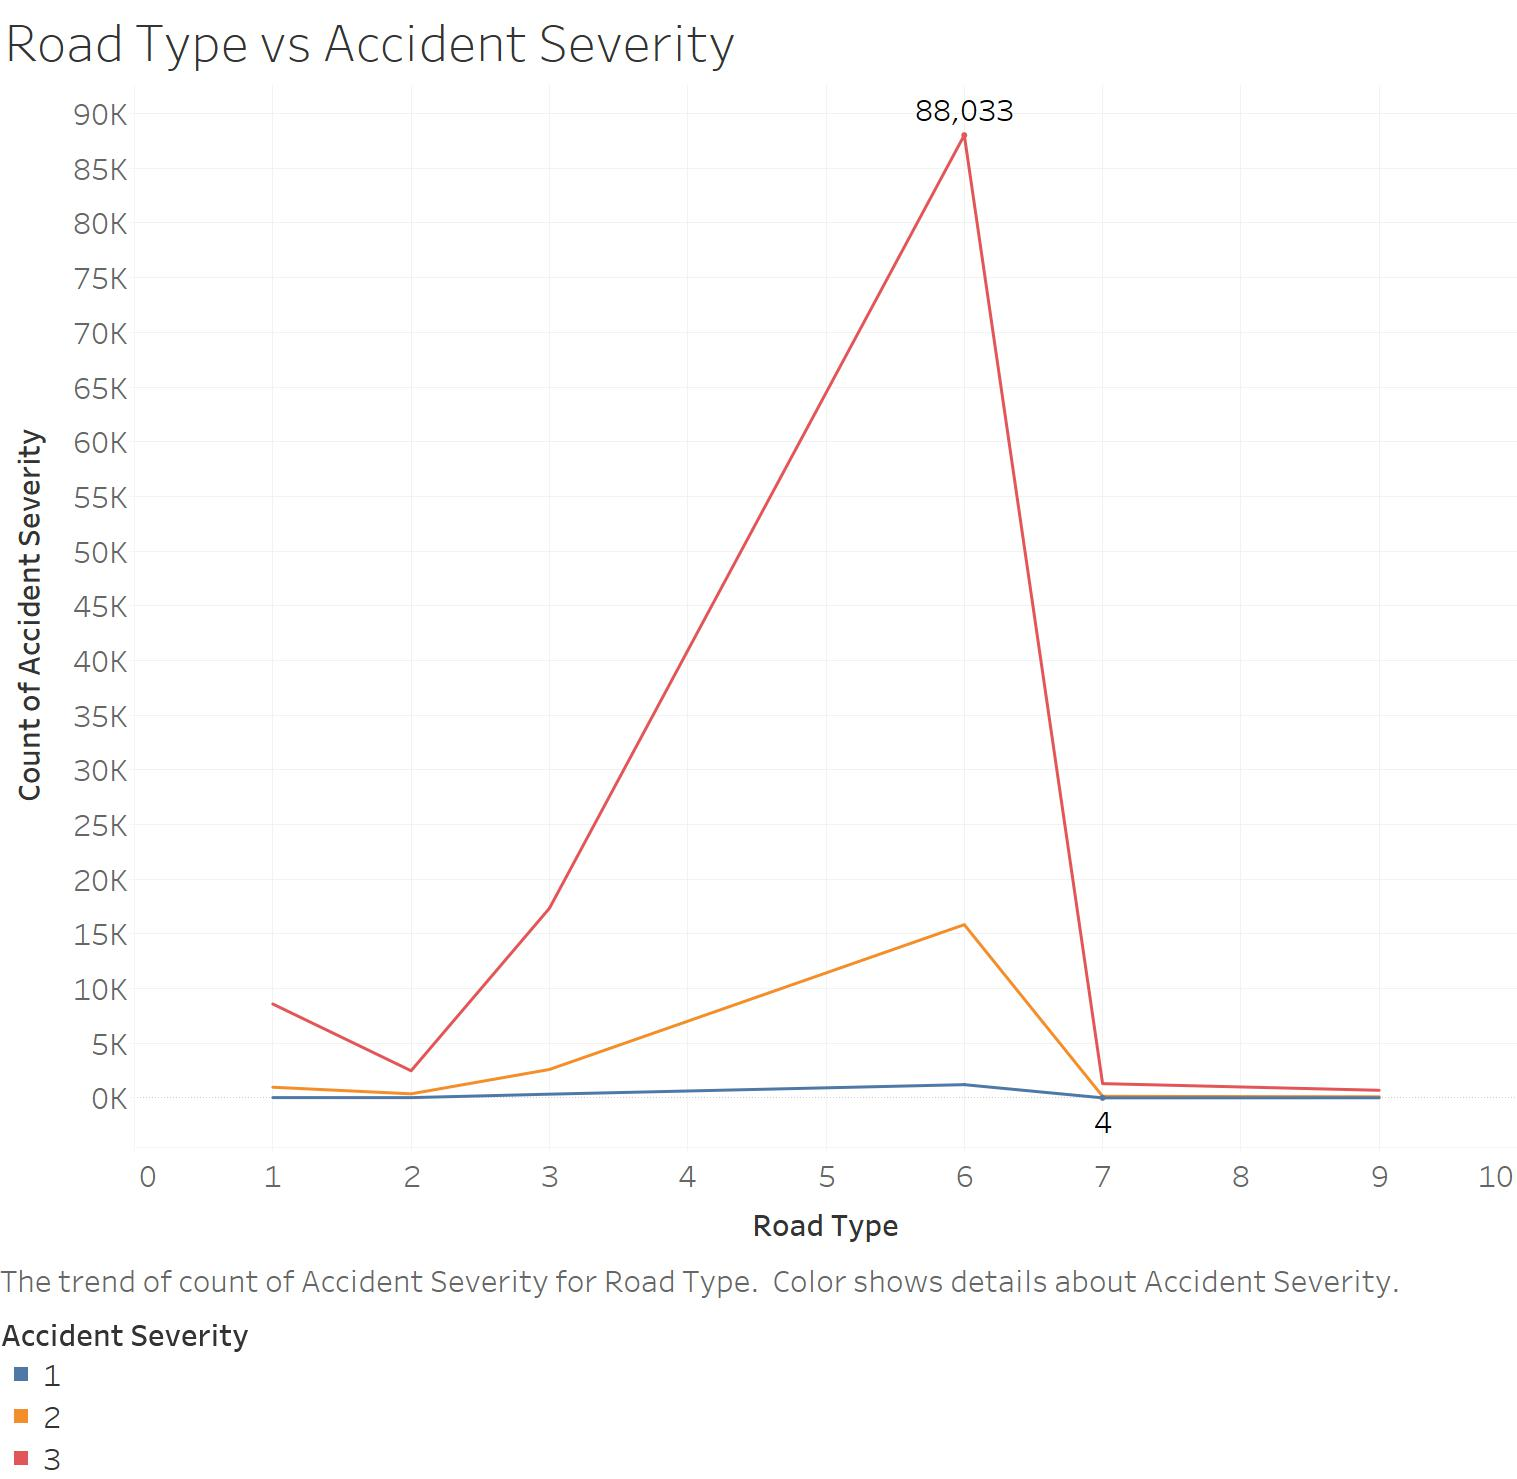
\includegraphics[width=1.0\columnwidth]{images/roadtype.jpg}
  \caption{Number of accidents occurred depending on the road type}
\end{figure}
The Figure 3 shows number of accidents occurred on when other conditions are applied. The conditions are:
0-None
1- Auto traffic signal out
2- Auto traffic signal partially defective 
3- Permanent road signing or marking defective or obscured
4- Roadworks
5- Road surface defective 
6- Oil or diesel
7- Mud \\
The Auto traffic signal was one of the other conditions when accidents occurred. This visualization can be helpful to overcome the problem of traffic signal and as a result, the number of accidents may get lowered.

The Figure 4 shows number of accidents occurred depending on the road type. The values correspond as follows: 
1- Roundabout
2- One way street
3- Dual carriageway
6- Single carriageway
7- Slip road
9- Unknown
The result shows that maximum road accidents for severity 3 occurred on road type Single carriageway.

\subsubsection{Plot of Accident locations in Google maps}
The Accident locations have been plotted in google map using API of google map.
 We have developed a simple web application using Python(Django) to accomplish this. With the help of Django module called geolocation, we have plotted the accident prone areas. We used the latitude and longitude coordinates to plot the map. This is an interactive web application in the sense that a user could click on the accident area and it would display the date and time of the accident occurrence. 

The accident locations with severity 1,2 and 3 are plotted on google map using google API in Figure 6, Figure 7 and Figure 8 respectively. 

%\end{itemize}


\section{Deployment}

\begin{figure}
      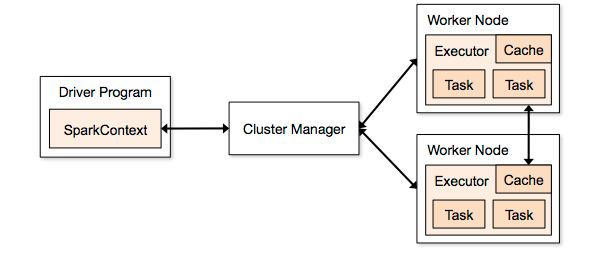
\includegraphics[width=1.0\columnwidth]{images/sparkarchitecture.JPG}
  \caption{Architecture of Apache Spark}
\end{figure}

\begin{figure*}
  \centering
      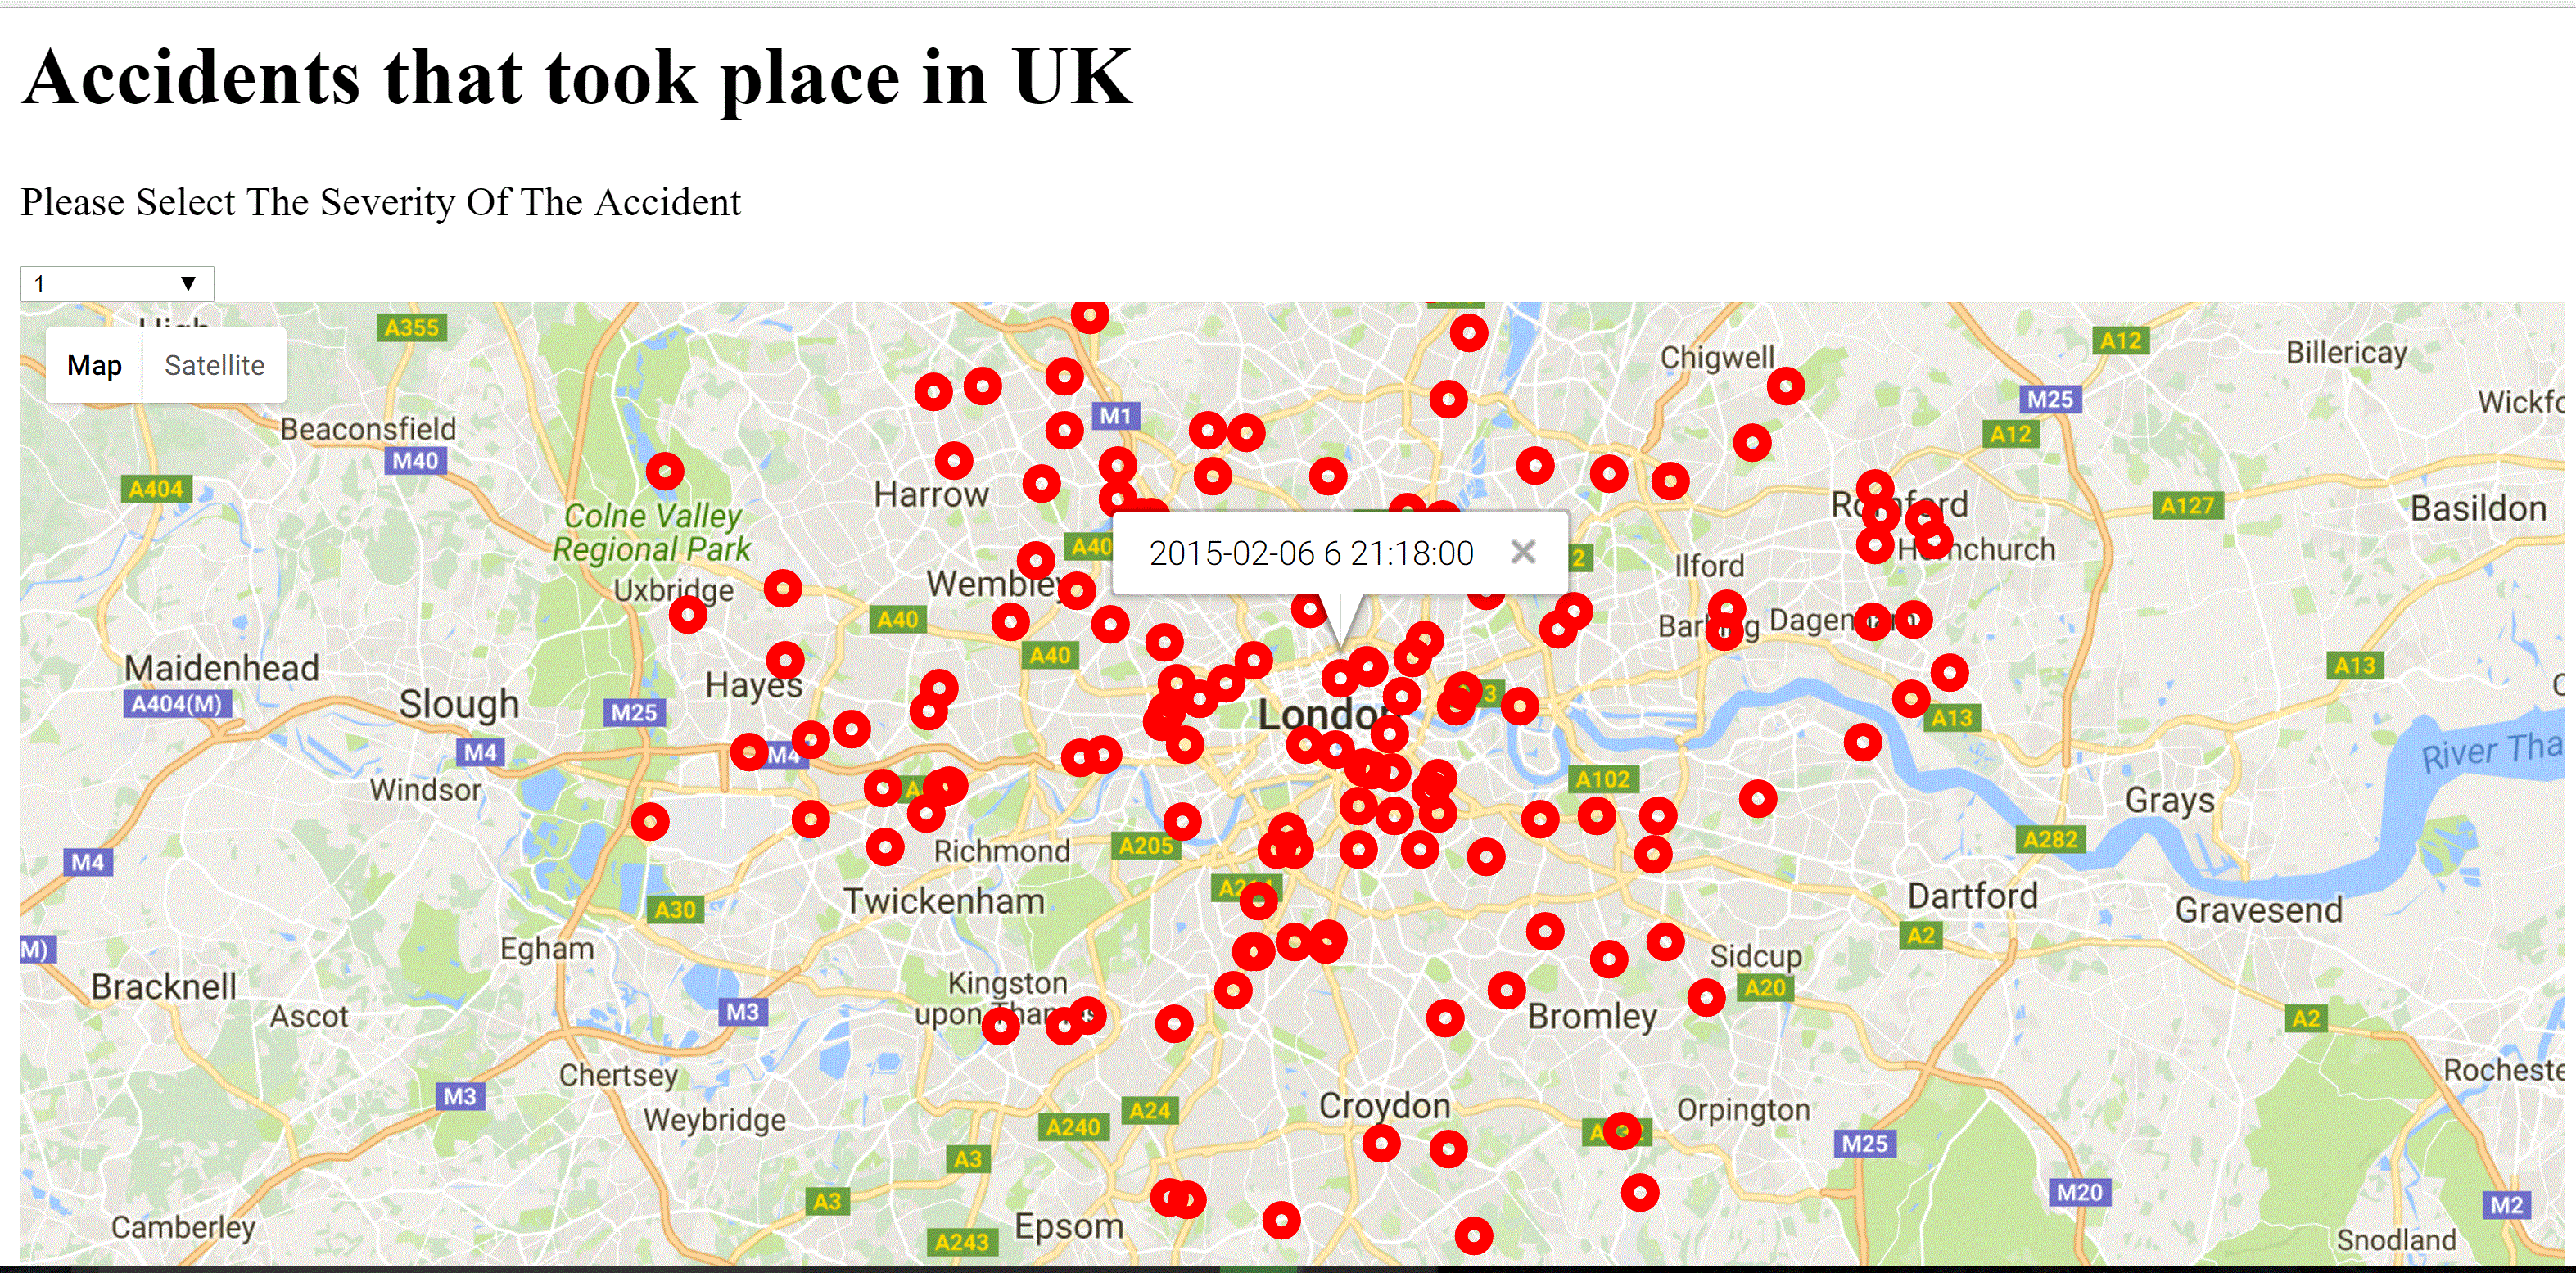
\includegraphics[width=1.0\textwidth]{images/googlemap.png}
  \caption{Google map displaying accident locations of severity 1.}
\end{figure*}


\begin{figure*}
  \centering
      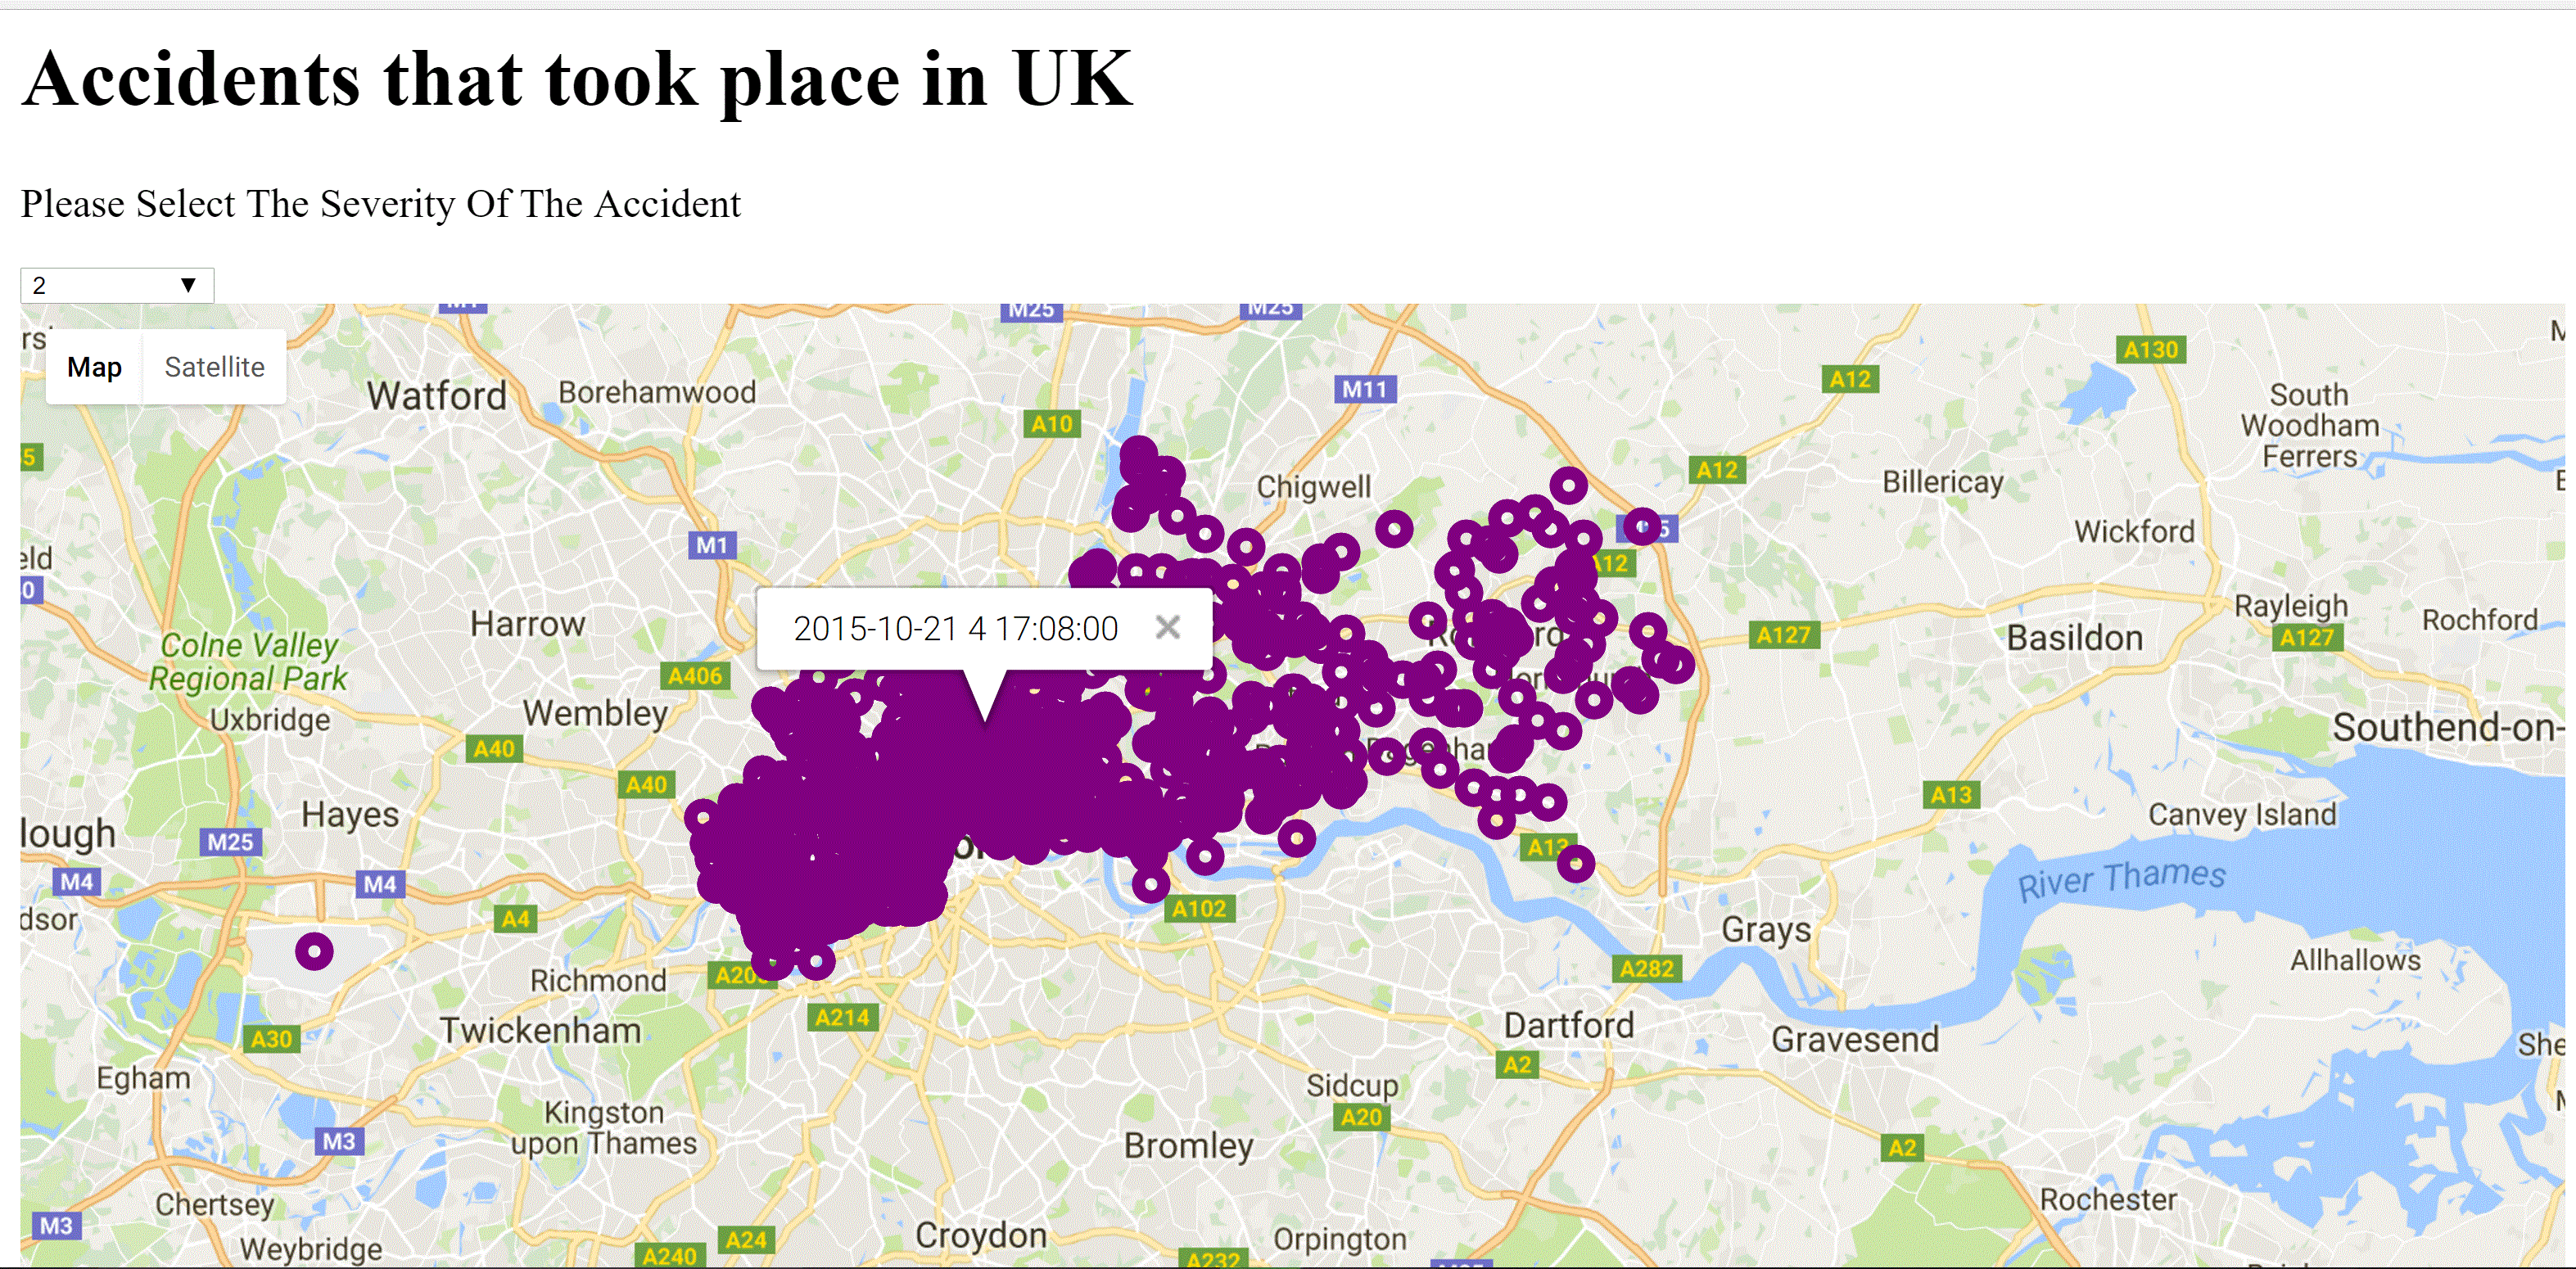
\includegraphics[width=1.0\textwidth]{images/googlemap2.png}
  \caption{Google map displaying accident locations of severity 2.}
\end{figure*}


\begin{figure*}
  \centering
      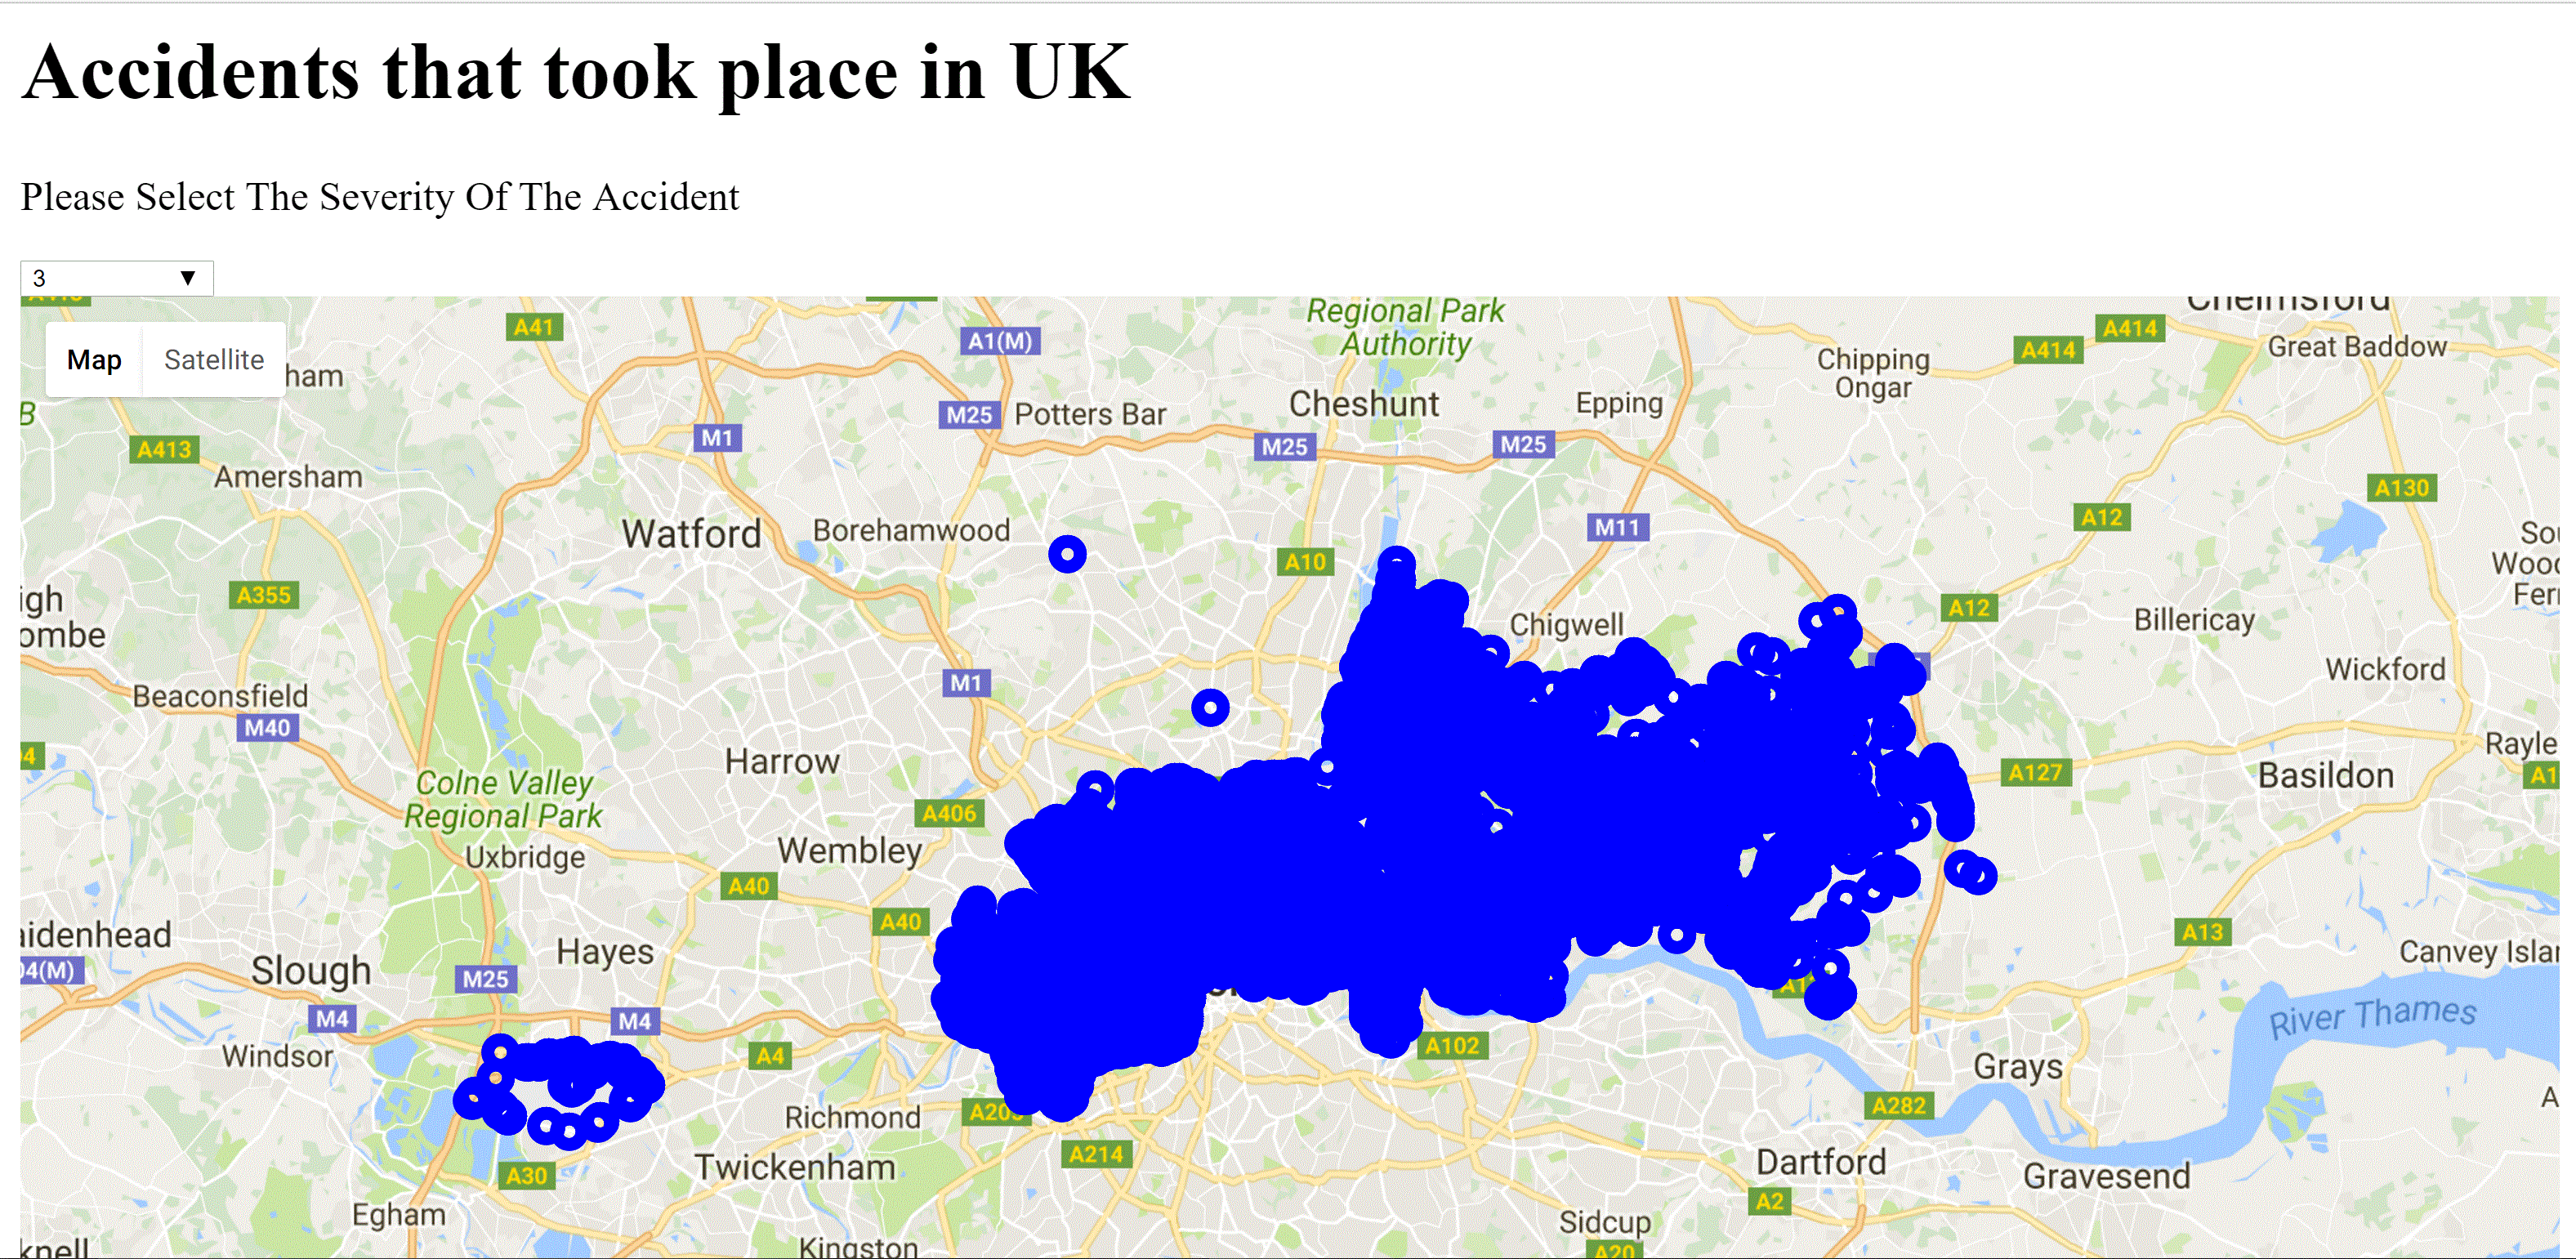
\includegraphics[width=1.0\textwidth]{images/googlemap3.png}
  \caption{Google map displaying accident locations of severity 3.}
\end{figure*}


We have used Databricks cloud for implementation of project. The community edition is used that comes free of cost.
Databricks provides a Just-in-Time data platform on top of Apache Spark that empowers anyone to build and deploy advanced analytical solutions.\\
Apache Spark is a fast and general-purpose cluster computing system. It provides high-level APIs in Java, Scala and Python, and an optimized engine that supports general execution graphs. It also supports a rich set of higher-level tools including Spark SQL for SQL and structured data processing, MLlib for machine learning, GraphX for graph processing, and Spark Streaming. \cite{apachespark}


Instructions on how to import Databricks notebook and run the code:

1) Go to https://community.cloud.databricks.com and sign up.\\
2) Select the Community Edition.\\
3) Sign up for Databricks Community Edition by entering personal details.\\
4) Select Workspace from the left-hand column, and under workspace, choose shared and select import under the dropdown.\\
5) Create Clusters by choosing the clusters in the left-hand column, click on the create cluster tab and enter the cluster name and Apache Spark Version Spark 2.0(Auto-Updating, Scala 2.0)\\


\section{Appendix}

For this project we have equally contributed for data analysis, code design and development, testing and all the documentation.

Kavya Guruprasad
F16-IG-3008:
Kavya was responsible for initial data set analysis. She created code for finding number of accidents and their severity during night time, number of accidents and their severity during night time and so on. Additionally, she visualized the location data in the data set and wrote the code for plotting on google maps. She created the Readme.rst file.

Nandini Goswami
F16-IG-3007:
Nandini was responsible to further clean and transform the data and do feature extraction.  Additionally, visualized data by writing python code and using Tableau.She helped in creating the readme.rst file. 

Sarita Bhateja
F16-IG-3003:
Sarita was responsible for converting the feature vector in a format that could be fed into the machine learning algorithms. She further ran the machine running algorithms and got the result. Also, she visualized data using Databricks.

We analysed the algorithm results and tried to evaluate which algorithm worked better.

\bibliographystyle{IEEEtran}
\bibliography{references}

%\balancecolumns 

\end{document}
